\subsection{Why does our system exist?}
In our research, we couldn't find a singular system that allows users to gain a
general overview of public amenities, for example, parking, bike infrastructure,
or public transport. In Ireland and the United Kingdom, the prevalence of proper
digitised records in county administrations varies wildly
(\cite{WebAccessibilityIreland}). Some make use of state-of-the-art geographical
information systems (GIS) while others rely on spreadsheets which are manually
kept up to date. (\cite{mcguirk2001changing})

\noindent{}A system that would allow users to quickly inspect a combined dataset
grounded in automatically generated, real-world data could accelerate processes
like planning permissions, urban development, or resource allocation. This
applies especially to smaller counties that may not have personnel experienced
in this area. (\cite{clark2002amenities})

\noindent{}Improving how governments allocates resources could lead to
improvements in efficiency, making public services more attainable, even for
smaller communities. For example, having accurate data on public transport and
bike infrastructure encourages more people to choose sustainable modes of
transport, helping reduce carbon and noise emissions (\cite{MUGION20181566}). It
could also make it easier for people in underserved communities to access
important services, such as housing, thus helping to bridge social gaps.
(\cite{allen2015understanding})

\noindent{}Currently, solutions are fragmented, focusing on just one type of
amenity, like transport or housing, without giving a full picture. Even the more
advanced GIS systems, while powerful, usually need a lot of manual input or
additional programming, which smaller municipalities or organizations might not
be able to handle. For example, to find parking spots in an area, the user needs to
either bring their own dataset or they have to perform computer vision analysis
themselves. While \textit{ArcGIS} includes tools to run deep learning on raster
images, the process is far from straight forward. Many of these GIS tools are also
expensive, or require specialised training, making them out of reach for smaller
boroughs or counties. (\cite{kaufmann2022scaling})

\subsection{The core technical problem}
The problem at the heart of our project is to find a way to collate and
visualize useful data about public amenities, without the need for any existing
information or manual data entry. This would allow the solution to be useful, no
matter the state of the users digital records. Relying purely on existing data
would do nothing to reduce the divide between counties with more data and
counties with less data. This necessitates the creation of an interconnected
series of modules that form a pipeline, for the automatic extraction and fusion
of data.

\noindent{}In order to present users with a map containing information about the
number of public amenities, we must first identify them. Our biggest technical
challenge is the extraction of these data points. Different forms of public
amenities exist in satellite imagery, we can combine this with other data
sources, interweaving them, and producing a better result.

\noindent{}Detecting public amenities from overhead views is a non-trivial process,
as satellite imagery suffers from low resolution, occlusion, seasonal changes, or
cloud cover. This means classifying specific objects can be complicated, and can
take a lot of time and processing power. For instance, the task of quantifying
on-street parking is dependent on reliably detecting cars that are not actively
participating in traffic (in aerial images). Not only that, but the detected
points in the images must be mapped back onto real-world coordinates to be of
any utility.

\noindent{}Ensuring consistency between the extracted data, and other data sets,
can have its own pitfalls. For example, compensating for:

\vspace{-3mm}
\begin{itemize}
  \item{different precision in geographical alignment}
  \item{varied update frequencies}
  \item{different data formats}
\end{itemize}
\vspace{-3mm}

\noindent{}Not only can data be geographically misaligned, but since satellite
data is only a snapshot in time, it can lead to temporal misalignment as well.
Even the appearance of amenities can change depending on their location. While
cars look more or less the same anywhere on Earth, the same cannot be said for
public transport links, housing or hospitals, which could lead to difficulties
achieving the same level of accuracy in different regions. Processing a large
amount of data like can be difficult and finding a strategy to do this
efficiently is necessary.

\subsection{A review of similar systems}

\noindent{}\textbf{Parkopedia}

\begin{figure}[h]
  \centering
  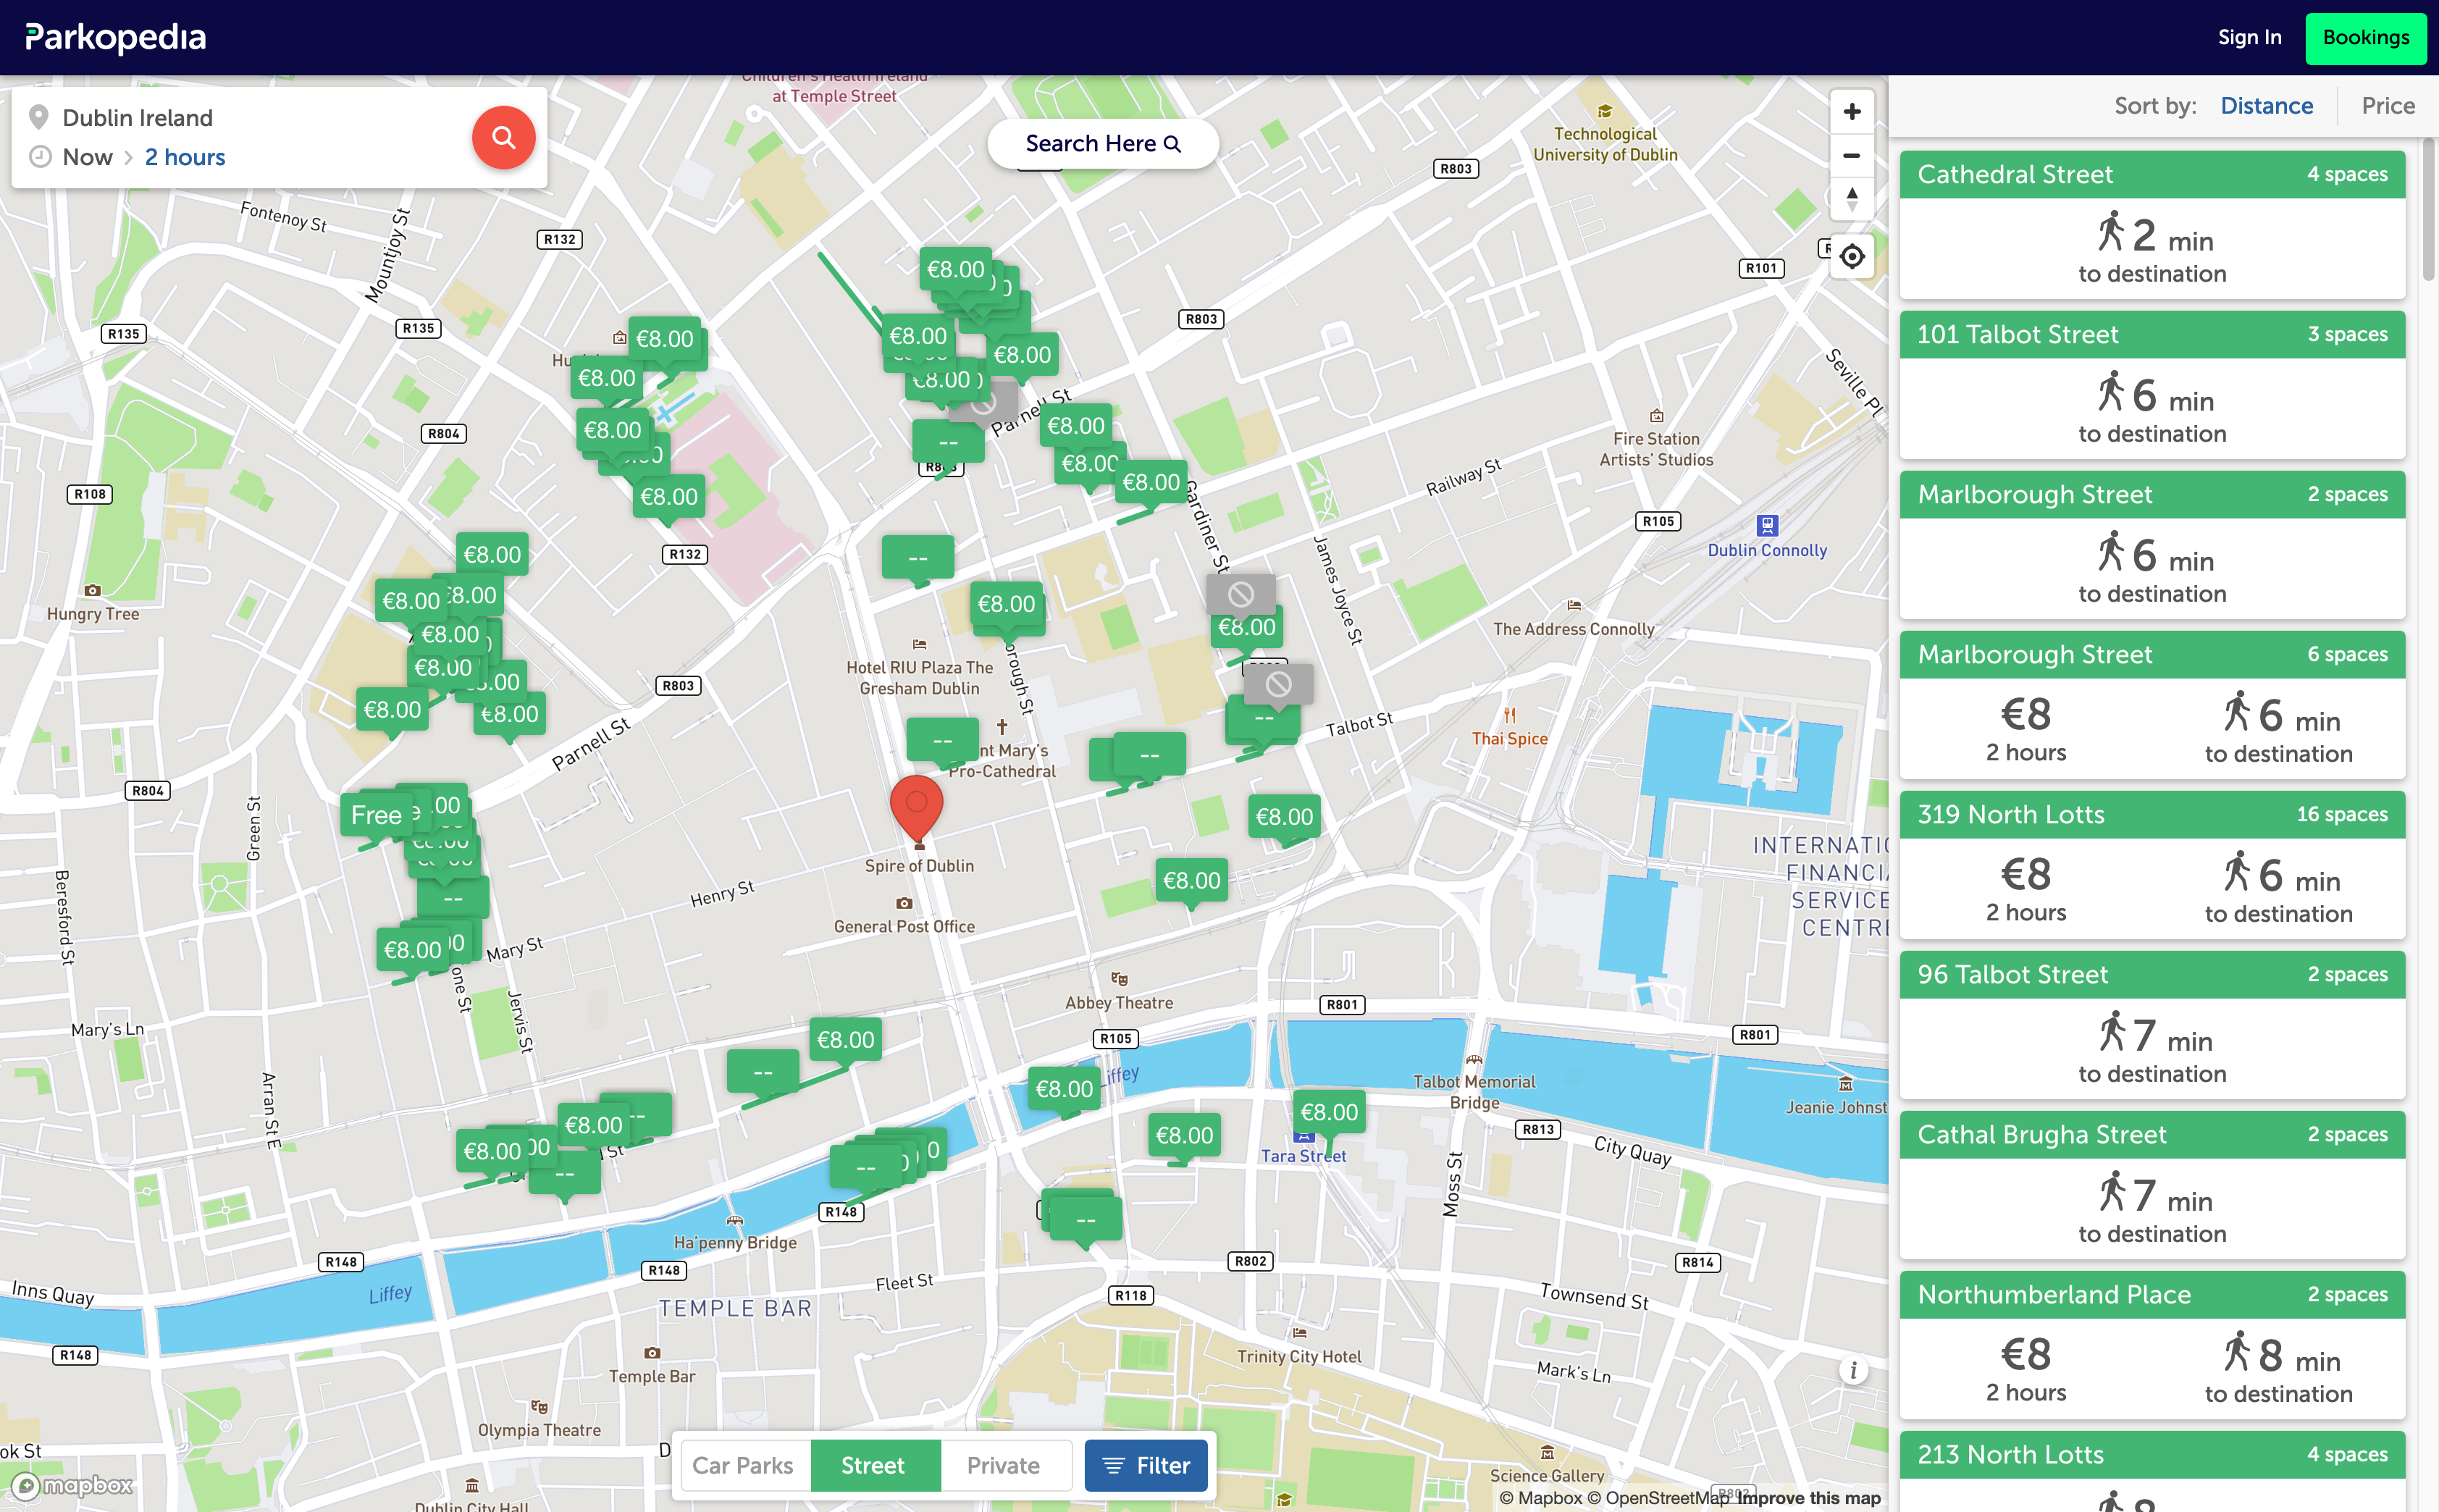
\includegraphics[width=\columnwidth]{images/parkopedia.png}
  \caption{Example of parkopedia}
  \label{fig:parkopedia}
\end{figure}

\noindent{}\textit{Parkopedia}\footnote{https://www.parkopedia.com/} is a web
application that allows users to find parking in many cities around the world.
They offer location and pricing data on parking garages, on-street parking and
parking on private property.

\noindent{}It is similar to \textit{Magpie} in the sense that it allows users to
gain a quick overview of all parking options in their area.

\noindent{}Our system differentiates itself from \textit{Parkopedia} in three
main ways:
\vspace{-3mm}
\begin{itemize}
  \item{\textbf{Data fusion:} Our system integrates data from publicly available
  sources, combining multiple datasets to provide a more comprehensive overview
  of public amenities -- not just parking.}
  \vspace{1.25mm}

  \item{\textbf{Aggregated data:} Our system offers a high-level overview of the
  amount of available amenities in a certain radius. This would be possible with
  the data from \textit{Parkopedia}, but the user would have to manually
  retrieve the data in which they are interested in analysing.}
  \vspace{1.25mm}

  \item{\textbf{No reliance on manual data entry:} Unlike
  \nobreak{\textit{Parkopedia}}, which relies on user-submitted information, we
  automatically acquire and fuse datasets. This pipeline allows us to keep
  information up-to-date and adapt our system to new regions without the need
  for manual data input.}
  \vspace{1.25mm}

\end{itemize}

\newpage{}

\noindent{}\textbf{ArcGIS}

\begin{figure}[h]
  \centering{}
  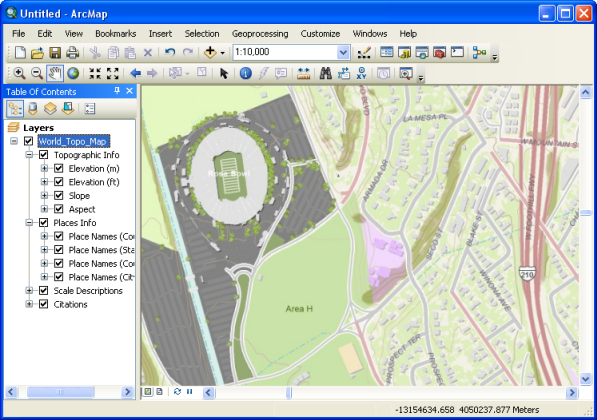
\includegraphics[width=0.85\columnwidth]{images/arcgis.png}
  \caption{Example of ArcGIS}
  \label{fig:arcgis}
\end{figure}

\noindent{}Systems like \textit{ArcGIS}\footnote{https://www.arcgis.com/} target
mainly expert users like cartographers and researchers. These systems are powerful
and feature-rich tools for professionals. While \textit{ArcGIS} is able to produce
the same overview offered by our system, it is different in these key aspects:

\begin{samepage}
\begin{itemize}
    \item{\textbf{Ease of use:} The goal of our system is to cater to a broad
    range of users, not just experts. Systems like \textit{ArcGIS} require
    specialised domain knowledge, as it's aimed at professional users. While
    \textit{ArcGIS} offers powerful tools, it can be overwhelming for the more
    general user who needs a quick overview of public amenities without engaging
    with advanced features.}
  \vspace{1.25mm}

  \item{\textbf{Accessibility:} GISs are a robust tool, but its access is often
  restricted lack of technical expertise. Compared to \textit{ArcGIS}, our
  system is less versatile. However, our system is more streamlined to offer- at
  a glance- an easily accessible way of gauging information about public
  amenities. This makes sure that users from all backgrounds can utilize our
  system without the need for specialised training.}
  \vspace{1.25mm}

\end{itemize}
\end{samepage}

\newpage{}